\chapter{Prototypische Umsetzung\label{chap5:Fuenftes-Kapitel}}

Anschließend an die Konzeption der prototypischen Umsetzung, erfolgt in diesem Kapitel eine Erläuterung der technischen Umsetzung. Neben einer Einführung in den Funktionsumfang des Prototypen, wird das Gesamtkonzept aus \autoref{sec4.3:Unterpunkt-3} in verschiedene Komponenten unterteilt.

% ToDo more Text

\section{Funktionsumfang\label{sec5.1:Unterpunkt-1}}

Der Umfang des Prototypen soll eine Bibliothek darstellen, in welcher ein Benutzer die Möglichkeit besitzt, Bücher anzulegen und zu verwalten. Hierfür werden die allgemeinen CRUD-Operationen zur Verfügung gestellt. Der Benutzer hat demnach die Möglichkeit neue Bücher dem Bestand hinzuzufügen (Create), sich den aktuellen Bestand anzeigen zu lassen (Read), bestehende Bücher zu ändern (Update) oder Bücher aus dem Bestand zu entfernen.

In \autoref{fig:UserInterface} ist die Benutzerschnittstelle abgebildet. Zu unterteilen ist die Ansicht in drei Bereiche \glqq Bücher hinzufügen/ändern\grqq{}, \glqq Aktueller Buchbestand\grqq{} und \glqq Suchfunktionalität\grqq{} untergliedert.

\begin{figure}[H]
    \centering
    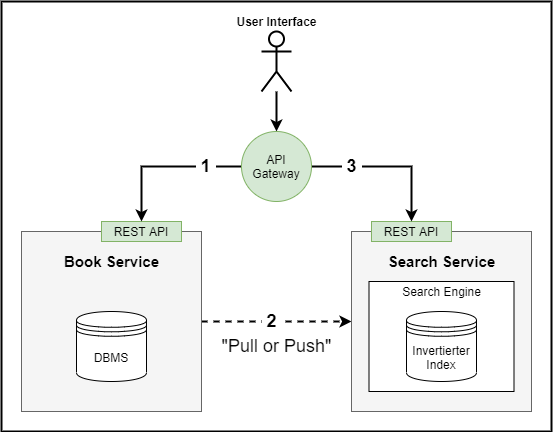
\includegraphics[width=0.9\linewidth]{images/pullpush_aktualisierung.png}
    \caption{Benutzeransicht der prototypischen Umsetzung}
    \label{fig:UserInterface}
\end{figure}

Im oberen Bereich haben die Benutzer die Möglichkeit neue Bücher dem Bestand hinzuzufügen. Durch Betätigung des Buttons \glqq Add\grqq{} werden die Informationen aus den darüberliegenden Feldern als neues Objekt in der Datenhaltung abgespeichert. Zusätzlich dient der obere Bereich der Bearbeitung bestehender Bücher. Hierfür wird im darunterliegenden Datenbestand das jeweilige Buch durch den Button \glqq Edit\grqq{} ausgewählt und die enthaltenen Informationen können anschließend bearbeitet und gespeichert werden. Durch Betätigung des Buttons \glqq Clear\grqq{} werden die Text- und Zahlenfelder geleert.

Der aktuelle Bestand der Bücher in der Datenhaltung, wird in einer Tabelle wiedergegeben. Angezeigt werden neben einer eindeutigen ID auch die Informationen Titel, Autor, Veröffentlichungsjahr, Sprache, ISBN und Zusammenfassung. Jede Reihe der Tabelle repräsentiert ein Buch-Objekt aus der Datenhaltung und kann jeweils durch den Button \glqq Edit\grqq{} bearbeitet oder durch den Button \glqq Delete\grqq{} entfernt werden.

Im unteren Bereich der Benutzerschnittstelle findet sich die Suchfunktionalität. Der Benutzer hat hierbei die Möglichkeit in das Textfeld eine beliebige Suchphrase einzugeben. Durch Betätigung des Buttons \glqq Search\grqq{} wird die Suchphrase an die Search Engine geschickt und die empfangenen Suchtreffer werden in der darunterliegenden Tabelle angezeigt.

Neben der reinen Eingabe einer Suchphrase könne auch Wildcards für die Suche verwendet werden. Unterstützt werden von Elasticsearch unter anderem die Wildcards \glqq ?\grqq{} und \glqq *\grqq{}. \glqq ?\grqq{} ersetzt dabei genau ein beliebiges Symbol, während durch \glqq *\grqq{} keine oder mehrere Symbol ersetzt werden.

Zusätzlich zu den Wildcards können auch die Attribute angegeben werden, über welche die Suche ausgeführt werden soll. Standardmäßig wird bei der Suche über alle vorhandenen Attribute gesucht. So ist es durch die Eingabe von \glqq status:active\grqq{} möglich, nach dem Begriff \glqq active\grqq{} in dem Attribut \glqq status\grqq{} zu suchen.

\section{Komponenten\label{sec5.2:Unterpunkt-2}}

Inhalt

\subsection{Book Service\label{sec5.2.1:Unterunterpunkt-1}}

Inhalt

\subsection{CDC-Datenpipeline\label{sec5.2.2:Unterunterpunkt-2}}

Inhalt

\subsection{Search Service\label{sec5.2.3:Unterunterpunkt-3}}

Inhalt